\documentclass[reprint,amsmath,amssymb,apr,aip,onecolumn, 11pt]{revtex4-1}
\usepackage[ruled]{algorithm2e}
\SetKwInOut{Input}{Input}
\SetKwInOut{Output}{Output\,}
\DontPrintSemicolon


\usepackage{graphicx}
\usepackage{graphics}
\usepackage{mathptmx}
\usepackage{times}
\usepackage{amsmath}
\usepackage{amssymb}
\usepackage{dcolumn}
\usepackage{bm}
\usepackage{units}
\usepackage{color}
\usepackage{soul}
\usepackage{multirow}
%\usepackage{algorithm}
%\usepackage{algorithmic}


\newcommand{\floor}[1]{\lfloor #1 \rfloor}
%\usepackage{xcolor}
%\pagecolor[HTML]{efefef}
\graphicspath{{figures/}}
\renewcommand{\baselinestretch}{1.00}
\newcommand{\pdfscale}{0.4}
\newcommand{\pdfscaletwocolumn}{0.37}

\bibliographystyle{naturemag}	

\begin{document}
	
	\title{Memory-Attention-Network (MAN) -- a concise model of mind}
	
	\author{Nandakumar Sasidharan Rajalekshmi}
	\affiliation{Independent researcher (sr.nanda.k@gmail.com)}
	

	
	
	\date{\today}
	\begin{abstract}
	Memory and attention have been identified as the main components of cognitive models. In this work, the memory is modeled as associative and is placed in a feedback loop with an attention network. Several functional aspects of the mind, including perception, logical thought, intuition, dreams, mind wandering, desire, emotion, and empathy, are explained using this simple structure. The model also gives suggestions on sources of attention deficiency and a possible path to mitigate them.
		
	\end{abstract}
	
	%	\begin{IEEEkeywords}
	%		In-memory computing,  Homomorphic encryption, Polynomial multiplication
	%	\end{IEEEkeywords}
	\maketitle
	\section{Introduction}
	
	
	
	\begin{figure}[h!]
		\centerline{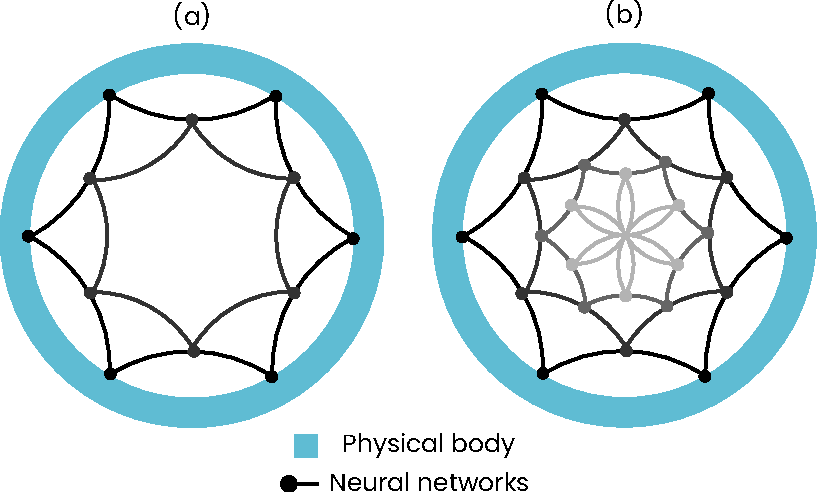
\includegraphics[width=0.65\linewidth]{figures/figure_man_animal_brain.pdf}}
		\caption{(a) An illustration of a system where the neural network layers are closely connected with the physical body to manage sensory and motor activities as expected in simpler organisms. (b) An illustration similar to (a) but with additional neural network layers which are not immediately connected with the physical body that allows additional memory and abstract representations. }
		\label{fig:man_animal}
	\end{figure}
	
	The uniqueness of the human brain is that it has significantly more layers of neurons that are not directly associated with various physical activities, such as sensory and motor activities, compared to simpler organisms\cite{2014_Hofman, 2011_DeFelipe} (Figure \ref{fig:man_animal}). This gives us additional memory that stores events over longer periods and allows us to compare and make associations among information that are not co-located in space or time. This enabled us to record patterns in our environment, predict the future based on past experiences, and plan strategies for desired outcomes. This additional memory and processing from the extra layers of neurons led to logical thinking, intuition, creativity, and more complex emotional responses. This memory of past experiences enabled us to successfully respond to new environmental challenges, made us curious about new possibilities and helped us to spread across the globe and to adapt to different climates. 
	
	
	
	The source of information for this memory has always been the experience of the person. It is important to note that the relation between memory and experiences is somewhat reciprocal\cite{Canli_2000, Tyng_2017}. That is, as our experiences formed memories, recollection of the memories was also able to recreate at least an impression of the experiences within the person.  When we realised symbols can trigger certain memories within us, we found a way to transfer experiences and knowledge of one person to another. This realisation gradually led to the development of symbolic languages. As a need arose to communicate information without physical proximity, and later as the amount of information accumulated started to grow beyond what we can hold in our memory, we started to note them down using symbols, on rocks, leaves, papers, and recently on electronic chips. As the accumulated information grew, it also helped us to develop new tools and methods to record them.
	
	As time progressed, we are now at a point where the tools being developed are capable of destroying the life as we know it. Today, several environmental indicators suggest that we might be doing it. It is puzzling that even when we are aware of the negative impacts, we find it very challenging to change the underlying patterns and habits. Hence, understanding the nature of the human mind, not just to manage diseases or to replicate in hardware for automation, but for a proper understanding of our behavior by everyone, is crucial for a peaceful coexistence of human beings and the survival of other species. This motivates the work here to formulate a model for the mind that is simple and concise enough for easy understanding, and at the same time sophisticated enough to capture the complex behavior of the mind. 
	
	Our attempts to understand the nature of the mind date back as far as our civilizations. The earliest work comes from the yogic sciences, which suggests methods to enhance attention, focus, and reduce mental activities, indicating that the exploration of the nature of the mind is ancient\cite{Vivekananda_1896}. Modern approaches depend on self-reflection, behavioral evaluation of willing participants, pathological evaluation of brain-damaged patients, and on neuro-imaging studies.  While there were times when we believed that the mind is separate from the body, today, it is widely agreed that mental activity is rooted in the human nervous system. The brain is the central seat of mental activities, but there are also embodied models of mind that demand the inclusion of the role played by the entire body in shaping perceptions. There are also extended and distributed models of the mind that attempt to include the group of people and the environment around the subjects for their role in shaping the mind. 
	
	Providing a comprehensive model for the entire mind has been challenging, and hence, some of the models have remained philosophical. Global Workspace Theory (GWT) is a prominent model for the mind that says that the conscious part of the mind is like the visible portion of a theater lit by a spotlight, though the activity there is influenced by other actors on stage,  audiences off stage, and directors behind the curtains. This metaphor is pointing to the fact that we are only conscious of thoughts that are at the center of our attention, even though they are influenced by a large volume of memory and processes originating from various sensory-motor signals and other physiological and psychological activities\cite{ Baars1988-BAAACT}. Integrated Information Theory (IIT) provides an abstract mathematical approach to measure the consciousness of any system, including our brain, as its capacity to integrate information\cite{ Tononi_2004_IIT}. As per this model, a higher degree of integrated information reflects a greater level of consciousness. 
	
	There is also a more evidence-based approach, focused on specific cognitive functions rather than aiming for a comprehensive model for the entire mind. Here we collect data, build mathematical models, and simulate and compare the results with human responses. This process iterates itself, creating more refined models.  This has led to the development of symbolic models, which include a collection of symbols and rules. ACT (Atomic Components of Thoughts), which later evolved to ACT-R (Adaptive Control of Thought-Rational)\cite{Anderson_1974, Anderson_1998}  and SOAR\cite{Newell_1990} are examples. They were designed to perform cognitive tasks, based on known facts stored in declarative memory and rules stored in procedural memory. ACT-R models their memory as associative and captures the limited capacity of attention by using buffers of limited size.  These models are more interpretable and are still being developed. Due to their need for hardware simulation, their lower-level architecture often mimicked the computer hardware of that time rather than the original biological systems.  
	

	The progress in neuro-imaging technologies towards the end of the 20th century helped us gain more concrete evidence and details on the general architecture, cellular structure, and signal patterns within the brain. The brain is composed of cells known as neurons, which are interconnected via junctions called synapses. These synapses are able to attenuate and delay the signal propagation through them. The brain is believed to learn, store, and adapt to situations by adjusting the strength of these synaptic connections. Connectionist models of the mind mimic this aspect of the brain. They implement cognitive functions using an array of interconnected artificial neurons. The connection strength of the neurons is adjusted gradually using learning algorithms to implement desired functions. Today's artificial neural networks (ANNs) come into this group. 
	
	The model I present in this work aims to bridge the gap between the specific cognitive models and the global models of the mind. It proposes a structure based on memory and attention in a feedback loop as a basic building block that can be replicated to perceive, record, and respond to different internal and external environmental inputs. Multiple channels of cognition come together in the brain, forming associations to build a more comprehensive model of the world. Then we explore how this architecture could be used to explain behavioral aspects of the mind, such as perception, logical thoughts, intuition, dreams, mind wandering, desire, emotion, and empathy.  Then we provide the neuroscience background and discuss the first-principle approach and the intuition behind the model. Towards the end, we also address some questions regarding the logical and emotional nature of the mind, how to enhance attention, memory, and consciousness. 
	
	

	
%	Uniqueness of human brain is extra layers of neurons compared to other animals.  The question is how do we organize this additional neural networks that can explain the nature of mind. From a survival point of view, the purpose of the mind is to observe and record the rhythms and patterns of its natural environment  and respond accordingly to keep the organism functional and alive. The response can be  in the form of either thoughts, symbolic communication, or physical activity. 
	
	
	\section{The Model }
	Let us first look at a few aspects of the mind that anyone can notice if we pay attention. 
	
	\begin{enumerate}
		\item Memory plays a central role in our mind. This memory stores impressions and experiences since childhood. 
		
		\item	The entire memory is not in our awareness all the time. What we pay attention to right now is what is in our awareness. 
		
		\item	We can pay attention to the thoughts from our memory,  sensations within the body, or sensory inputs from outside.
		
		\item	What we pay attention to, gets recorded in our memory.  
		
		\item	Moments or events of emotion, interest, or desire are easily recorded in memory. Repetition also helps to enhance memory.
		
		\item When we  focus on an object, we tend to remember information related to that object.  
		
		\item	Our thoughts are made of memories that we collected through different forms of experiences. 
		
		\item	The capacity of our attention is limited. 
		
		\item  When our attention is focused on thoughts and imagination, we become partially blind to the signals coming through other sense organs.
		
		
	 	
%	 	\item	Our ability to recover a specific information from memory depends on placing an appropriate query in our attention. The memory responds with associated information. This new information comes into our attention and it also becomes a  query to the memory to extract the next piece of information. This continuous feedback can create a train of thoughts.  
	 	
%	 	\item If we encounter something that we cannot relate with any of our previous memory, for example let us say a new word in a new language, it will be recorded in the memory, but we may find it difficult to recover, because we do not have an associated query. In  this case the word itself becomes the query. When we hear it again, the memory responds indicating that we have heard the word before. 
	 	
	 \end{enumerate}
	
	
	
	\begin{figure}[h!]
		\centerline{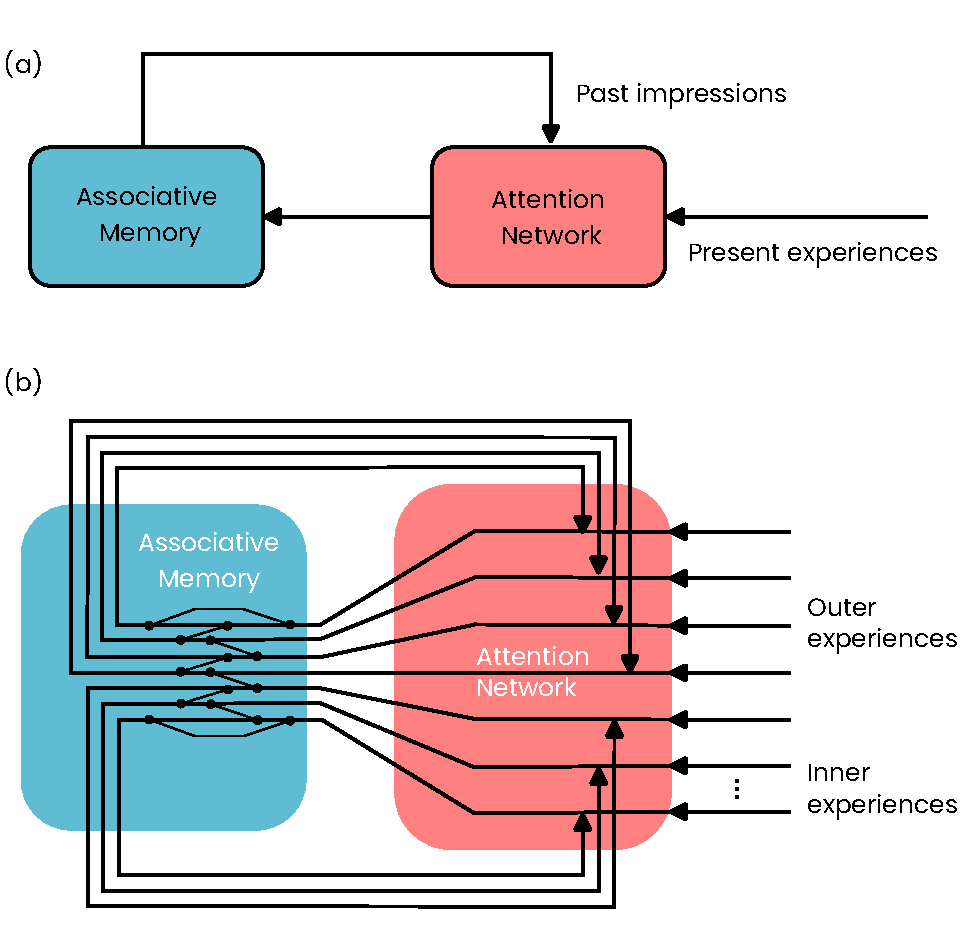
\includegraphics[width=0.8\linewidth]{figures/figure_man_model.pdf}}
		\caption{(a) The model for the mind where the memory and attention are in a feedback loop. Attention network is a combination of attention channels dedicated for signals from different sources. Present experiences denotes a combination of  the signals received from sense organs (Outer experiences) and sensations within the body (Inner experiences). What passes through the attention channel becomes input to the memory. The memory is modeled as associative memory, which records its inputs in an associative manner. When the memory is probed with a known input, its output  (Past impressions) help to give context and meaning to the inputs of attention. (b) A simplified line diagram of the model. The attention channel is modeled as a combination of multiple attention channels that acts as pathways for signals from both inside and outside the physical body. The information from different channels are recorded in the memory in an associative manner. }
		\label{fig:model}
	\end{figure}
	
	To capture these aspects, I construct a structure referred to as a memory-attention-network (MAN). This model of the mind has an associative memory (AM) and an attention network in a feedback loop (Figure \ref{fig:model}(a)). The nature of the memory modeled as an associative memory is to respond with related information when presented with an input. If any part of the AM holds information that matches its input, the memory first responds with a complete or partial replica of the input. This gives a sense of familiarity and helps us recognize familiar objects even from partial inputs by auto-completing them within the mind. Upon sustained attention, the AM activates related information, which gives a sense of knowledge and methods to respond to the input appropriately. If the memory finds no match for the input, it will attempt to replicate the input, which results in the storage of the new data. The data will be recorded in association with other related information, such as previous data points in the same sequence or the context provided by inputs from other sense organs. The different impressions and related information provided by the AM in response to an input are referred to as past impressions.     
%		
		
		 Attention network can be viewed as a combination of attention channels, each with its capacity limits on the number of items that can pass through at a time (Figure \ref{fig:model}(b)). Each channel carries signals representing present experiences originating either from the sense organs (outer experiences) or the sensations within the body (inner experiences), such as emotions,  pain, hunger, and (un)pleasantness. The signals that pass through the attention network reach memory. An input to the AM evokes its response (past impressions), and this becomes an additional input to the respective attention channels. Therefore, each attention channel has two inputs: present experience and past impressions. The attention channels can choose to focus on the present information, the memory response, or on a combination of them. 
		 
		 
		 If the attention is focused on the present experiences, it maximizes the information inflow from the current situation. This helps in gaining new experiences, memories, and learning. This phase could be slightly more energy expensive since the memory is integrating new information. If the current situation is familiar, we can work with partial or sparse external input, autocompleted by the memory responses to save energy. Here, the attention will be split between present experiences and past impressions.  Now, if the attention is focused on the memory response, it completes the feedback loop and leads to a train of thoughts. Due to the limited capacity of the attention channels, this `lost in thoughts' state will fully or partially block the channels from accepting signals corresponding to the present experiences. This feedback loop can also aid in memory reinforcement by repetition and in developing abstractions, intuitions, and imagination.   

		
	The AM is assumed to have a large capacity and a long data retention period. The different signals coming through the same attention channel are stored in the AM based on their similarity with each other in a physically closer space. This type of data recording leads to compartmentalization within the memory. While the signals from different channels get stored in physically separate spaces, they still record the association among them using dedicated neural connections. For example, depending on whether you are at home, school, or the office, you expect a certain combination of vision, sound, smell, and feel, unconsciously. You would generally notice if one of the sense inputs does not match the rest. Now, if one of the attention channels completes the feedback loop by focusing on the memory output and generates a thought sequence, it could potentially evoke associated memory from other channels, and they could obstruct the corresponding attention channels as well.
	
	
		
		
		 
%			\begin{figure}[h!]
%			\centerline{\includegraphics[width=0.6\linewidth]{figures/figure_comparison.pdf}}
%			\caption{Associative memory versus standard digital memory. Associative memory when probed with information finds the closest match from its records and outputs related information. On the other hand, a standard digital memory will output data stored at an exact location when probed with the corresponding address.}
%			\label{fig:compare}
%		\end{figure}
	
		

\section{Functioning of the model}
%In the sections below focus primarily on how the model functions. Its neuroscience can be discussed later. 
In this section, we discuss how the model can be used to explain different behaviors of the mind. 



\subsection{Perception, memorization and learning}

In the model, what passes through the attention network is what we perceive. The corresponding response of the memory helps us associate them with past impressions, giving them names and contexts. For example, if we hear the word `flute', either a picture or a sense of its sound or both comes to the forefront of attention, giving us a feeling of recognition. 

When the model encounters an unfamiliar signal, the memory fails to respond with a matching past impression. This maximizes the available attention bandwidth for the new input. Now we receive the input with maximum details, and the AM will attempt to create a `past impression' signal by replicating its input. This process will form a memory of the input. Once again, this new record will be formed in association with other familiar objects, symbols, sounds, or experiences which are adjacent in time or space. This way, the memory does not form isolated impressions, but rather meaningful sequences. 

In addition to the memory that we acquire from outside, our body also carries a large amount of memory in the form of genetics. This innate memory modifies our priorities and learning behavior through survival instincts. We experience the survival instincts in the form of different sensations within the body. Events that generate these additional inner experiences ((un)pleasantness, emotions, pain, pleasure) via additional awareness channels have a chance to form more associations and hence lead to stronger memories. In events that lead to fewer or no inner experiences, the chances of attention focusing on the memory response are higher, completing the feedback loop of distracting thoughts. Hence, such events will need more effort to attend to and will need more repetition to form an equally vivid memory.

For a human baby, mimicry is the easiest way to learn. They learn to walk and talk by observing and mimicking their parents. Later, they acquire decision-making skills from their collective experiences. For example, the survival instincts of a newborn baby prompt it to cry when it feels hungry. The baby gets fed, and the physical experience signals satisfaction. The memory records this successful sequence, and the memory will trigger this sequence again even at the slightest indication of hunger in the body.  Now, over a period of time, the child's memory will accumulate a collection of successful and unsuccessful action sequences to choose from to meet its physical needs depending on the varying responses of the parents. The model can capture these behaviors. 


\subsection{Abstraction, Logical thinking and Intuition \label{sec:abs_intuition}}

 Abstraction  is a process that determines the most essential features from several examples. Let us examine it using a physical situation. If I drop a stone, it will fall to the ground. If I drop a cup, it will fall to the ground. If I drop a ball, it will fall to the ground. These are all true in my observation and experience. The AM does not need to store all these three instances as independent sequences. Falling to the ground is common among these three objects. As I gain experience with more objects, the mind detects a feeling of heaviness in the hands as a common factor. Now, the AM can form an association between the feeling of heaviness and the fall when dropped. With additional experiences, the mind may detect that, however light, almost all objects fall to the ground when dropped. The associative nature of memorization and the ability of the AM to respond based on similarity will naturally extract the essential features from repeating situations and ideas, which we refer to as abstraction. 
 
 What is true in our experience is what we consider logical. In other words, if something happens as we expect, we will consider it logical. If the result of a sequence of events matches what is predicted by our mind, we perceive it as logical. Here, the source of our prior knowledge or experience could also be indirect, where the experience of another person received via communication is accepted as true. What is logical can also be deduced by combining smaller logical facts or events.  Let $A->B$ ($A$ implies $B$) and $B->C$ be two independent logically true statements for a person. If these two statements are recorded as sequences within the AM, because of the feedback structure in the model, it will naturally deduce the transition from  $A->B->C$.  If the mind encounters this sequence repeatedly, it may learn a direct relation between $A$ and $C$ and will produce $A->C$ without the intermediate step $B$, which we interpret as intuition. 
 
 Essentially, the model suggests that the mind is replicating the outside world in its memory, runs the sequence through the attention-memory loop during thoughts or memory consolidation processes, forms logical ideas, forms higher-level associations, and gradually develops abstractions and intuitions. 
 


\subsection{Emotion and empathy}
The range of emotions expressed by a human being is not always constant. A newborn baby's emotions are primarily reflexive, such as crying or contentment, driven by hunger, sleep, etc. As the baby gradually grows to an adult, the range of emotions expressed also increases\cite{Berk_2017}. This shows that as we accumulate more experiences, we become capable of more complex emotions. Barring the impact of brain development, we look at how the model captures this scenario. The relation between memory and experience is somewhat reciprocal. As experiences create memories, the recollection of these memories is also capable of affecting the experiences within the system. For example, if a particular sequence of events has led to pain in the past, in the future, when a similar situation starts to happen, the model will automatically start to project the painful outcome. The body will experience this expectation as fear or anxiety. If the outcome in the past was pleasant, in the future, the body will experience excitement in expectation. Similarly, physical experiences from the past projected into the future will create different emotional responses.

Empathy is our ability to experience and relate to other people's mental and emotional states. The model that records external sequences and corresponding inner experiences in association will be able to capture this behavior. As we observe someone going through a difficult situation, the model will be able to recall a similar sequence from our memories. This will automatically evoke at least a mental impression of similar physical and emotional situations within us. This ability to recreate another person's inner situation within ourselves, by virtue of our mind's character to mimic, produces empathy.  

\subsection{Ability to ask question}
Our ability to ask questions potentially originates from our ability to predict events, based on memory. Our success in prediction is also recorded as a sequence that careful observation leads to successful prediction and new knowledge. Now, when we encounter an event that we are not able to predict, we start a process of more careful observation. This phenomenon, when expressed using languages, we call it asking questions. Hence, our model that stores sequences can potentially evolve the ability to ask questions. 

\subsection{Symbolic language and language learning}

Language at a very basic level is a collection of sounds/symbols used by a group of people to communicate about the world around us. The association between symbols and objects or events can be stored in an AM and easily retrieved. The model-based sequence generator can also generate the control signals to produce the sounds for speech (see also section \ref{sec:Generalization}). Initially, a small group of people would have used symbols to communicate, which increased their coordination and success rate in the survival process. Others' minds can make the association between language use and the success rate of this group, and will start to copy their behavior of using sounds/symbols to represent objects and ideas, leading to a wider adoption of language. 

\subsection{Desire}
Desire originate from a difference between an  actual experience and a mental impressions of the same. For example, when you see a sweet dish, you remember how wonderful it tastes, but it is not same as the actual experience of eating it. Now you feel a certain urge to eat it to recreate the original experience. It is also possible that you may not have ever eaten this particular sweet, but have heard about its wonderful taste from a friend. Once again this memory obtained via a secondary source creates an urge to realize it in actual experience. 

The following aspects of the model helps implement the process of desire.  The AM can record the difference between hearing about an experience or a memory of it and an actual experience since all of them are active at the same time. Once you see the object of desire the AM in feedback loop will constantly bring up the associated memory creating a certain fixation of attention on the object. The ability of the memory to record sensory experiences from inside the body is another factor that helps generate desire. 





\subsection{Goal oriented behavior}
Our goal orientation is driven by survival instincts and desire. We seem to be engaging in activities which does not seem to be triggered by any of the cues in our immediate surroundings. How can the model explain this behavior? Our memory is probed not just by external sensory inputs, but also by our inner experiences. Here, our survival needs such as hunger, thirst, etc, will constantly remind us of the actions needed to saty alive and desires will remind us of the actions needed to increase the experiences in life. The duties we take up and the goals we set are different strategies we have developed over time to meet the primary survival needs. The plans we set and strategies we design are based on our own trial and error experiments, or acquired via observation, reading or other means of communication. We may also unconsciously draw examples from different histories and stories we have read. Accordingly, our mind produces a sequence of actions or a pattern of activities, expecting a positive outcome. Our model with AM in a feedback loop with attention networks can potentially build such action sequences.  

\subsection{Creative thinking and imagination}
Creative thinking and imagination are processes where relatable ideas, visuals or symbols are put together that were never related in actual experience. The ability to form abstractions and to ask questions helps the model to put together pieces of information that were never actually together. Here, the question is instead of `why' it is `why not'. As we discussed earlier, when the AM is presented with different examples of similar objects or events, it tends to form associations between their abstract characteristics. This association at the abstract level happens naturally due to the characteristics of the AM to always store new content based on its correlation with the existing content. During imagination, the associations formed at the abstract levels act as bridges that permit switching between different examples. 


\subsection{Mind wandering and dreaming}


The fundamental mechanism behind thinking, mind-wandering, and dreaming is essentially the same, though the contexts in which they happen are different. All of them are a sequence of interconnected impressions in the memory passing through your awareness. The AM in a feedback loop with the attention network can capture the basic mechanism behind all of them.  Thinking is a more active process that happens while awake, often to find a solution to a real-world problem. Mind-wandering is a more passive process, happens while awake, and is the free running of the feedback loop. Both of these happen while awake, and the body provides sufficient cues, making them more physically realistic. 

Dreaming is mind-wandering while asleep. It may be triggered by recently active memory, emotions, or other noise. During sleep, there is a brain-body disconnect\cite{Jones_2018}, and certain parts of the brain become less active, reducing the physical contexts and cues, making the dreams more imaginative. As the content of the memory passes through the attention network, it may also arouse emotional responses like fear, anxiety, pleasure and joy. For example, suppose you are working under stress from time constraints. Now, when you go to sleep, the work-related thoughts could still be active. The mind will capture this emotion at an abstract level and will activate associated experiences from the past. The feedback loop will build a cinema using the associated pieces. Now you may dream of running to reach somewhere on time, or trying hard to finish an exam on time, but never really getting to the end point. As you go through the dream, you will once again experience the stress. Recording experiences in an associative manner within the MAN model can potentially recreate this scenario. 


\subsection{Generalization \label{sec:Generalization}}

\begin{figure}[h!]
	\centerline{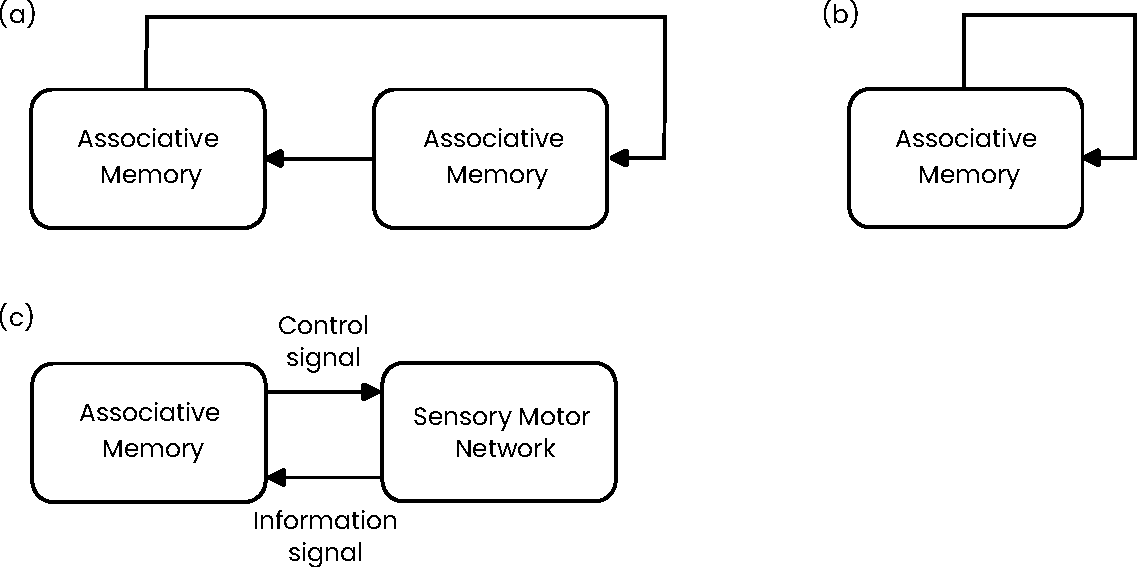
\includegraphics[width=1\linewidth]{figures/figure_model_generalization.pdf}}
	\caption{(a) Associative memories may potentially cascade with each other to copy information from one region to another or to generate more complex sequences. (b) An AM circuit that forms a feedback loop around itself without the attention network. (c) The AM may also interface with the sensory motor network, which interacts with the musculoskeletal system to learn and generate the necessary control signal for various physical activities. }
	\label{fig:model_generalization}
\end{figure}

Organising the neural circuits as associative memory has several benefits. From a survival point of view, the AMs could be a good candidate that can record and respond to external situations without any additional control logic. Its simplicity makes it amenable to being replicated in several roles. We discuss some possibilities here. An AM-like organization allows different neural circuits to talk to each other. It could copy information from one region to another or make more complex thought processes (Figure \ref{fig:model_generalization}a). The AM may feed back around itself without the intervention of the attention networks (Figure \ref{fig:model_generalization}b). This could be helpful for memory consolidation. Memory consolidation is a process hypothesized to happen during sleep, which causes the replay and repetition of fresh memories and helps to enhance their retention\cite{Diekelmann_2010}.  The same AM-based memory model can also be used to generate control signals for various internal and external physical activities, such as rhythmic functioning of the organs, speech, locomotion, and limb movements (Figure \ref{fig:model_generalization}c). When we learn a new activity, it require deliberate attention. However, with regular practices, we tend to gain a certain expertise where the sequence of operation could be executed with  minimum attention. The memory structure in Figure \ref{fig:model_generalization}c could be employed to model this situation. 



\section{Neuroscience background}


We gained early insights into the anatomy of the brain by successfully associating cognitive deficits with localized brain damage (lesions). Wernicke's aphasia, a language disorder with impaired comprehension of spoken and written language and with fluent but often nonsensical speech, is an interesting example. Carl Wernicke's deduction in this case gave insights into the language comprehension mechanism in the brain. Wernicke's area in the left temporal lobe lies next to the cortical area for hearing, and this area was assumed to be involved in spoken language recognition. Broca's area in the frontal lobe lies close to the region responsible for the motor representation of organs of speech such as the face, tongue, lips, and vocal chords. A nerve bundle known as the arcuate fasciculus serve as a communication highway between these areas. Wernicke established the nature of the association between these two areas. Language learning and comprehension begin in the spoken format. Articulation and writing skills are secondary skills that we gain in association with primary comprehension skills. However, the signals for articulation are memorized in Broca's area. Now, a damaged Wernicke's area impaired language comprehension, but left the skill for speech intact. However, without the associated comprehension, the speech became nonsensical. Later, Wernicke's insights helped predict the impacts of several brain lesions correctly. This work also established that similar data were stored together and in association with prior supporting knowledge, leading to a compartmentalization in the brain; at the same time, these different regions can develop associations to perform more complex activities.  



However, the resolution and reliability of the lesion studies were limited. Later functional imaging techniques, such as electroencephalography (EEG), positron emission tomography (PET) and early functional magnetic resonance imaging (fMRI) allowed us to monitor brain cellular activities with higher resolution. Based on early lesion studies, neuro-images and behavioral analysis, psychologists started to model the brain into separate memory and attention regions, which were then used to design experiments to identify corresponding brain regions with higher accuracy. However,  due to the associative nature of data storage, one region might be active during several cognitive tasks, and hence isolating the specific role of each region is quite challenging. Hence, brain characterization involves a certain iterative refinement, where available data is used to create models and hypotheses that become the basis to design new experiments, and the process is still ongoing. 


Below, we look at some evidence of the attention network and the models of memory provided by neuroscience and psychology. 

\subsection{Attention network}

In The Principles of Psychology, William James describes attention as ``the taking possession by the mind, in clear and vivid form, of one out of what seem several simultaneously possible objects or trains of thought"\cite{James_1890}. James distinguishes between voluntary and involuntary attention and discusses the capacity limits.  Helmholtz’s work on visual attention, the ability to shift focus within the field of vision without moving the eye, suggested involvement of neural mechanisms for prioritizing sensory input\cite{Helmholtz_1925,Carrasco_2011}. 
The filter theory of attention proposed by Donald Broadbent suggests attention as a limited capacity system to effectively manage sensory overload based on experiments like dichotic listening tasks\cite{Broadbent_1958}.

Experimentally establishing that the neural mechanism behind attention is distinct from that of memory is challenging since both of them could be distributed across multiple brain regions and be active simultaneously. Early evidence came from lesion studies and behavioral observations. Hemispatial neglect, where patients with parietal lobe damage showed a disability to respond to stimuli from one side of the space, without a memory deficit, suggested a separate neural mechanism\cite{HEILMAN1977, VALLAR1986}. Another set of studies evaluates attention using reaction time, which seems to vary based on the time of the day following a circadian rhythm\cite{Matchock2009, BLATTER2007}. Pharmacological interventions that selectively target neurotransmitters in the attention-related brain areas such as the prefrontal cortex (PFC), anterior cingulate cortex (ACC), and dorsal attention network (DAN) and seem to enhance attention without affecting memory, are also indicative of separate neural mechanisms\cite{SPENCER2000, Scahill2001}. 


A more formal structure for the attention network comes from Michael Posner and Steven Petersen. They derived three subsystems for alerting, orienting, and executive control, which they mapped to different brain regions based on a combination of behavioral, lesion, and neuroimaging data.  Alerting was linked to the locus coeruleus and frontoparietal regions. Orienting was associated with the superior parietal lobule, temporoparietal junction, and frontal eye fields. Executive control was tied to the dorsolateral prefrontal cortex and anterior cingulate cortex\cite{Posner_1990}. Later, they developed an Attention Network Test to evaluate the efficacy of these subsystems based on reaction times, and their study suggests these subsystems are functionally independent\cite{Fan_2002}. A more recent study suggests these attention subsystems also recruit partially overlapping brain networks\cite{Markett_2022}. 





%The advent of functional MRI (fMRI) and positron emission tomography (PET) in the 1990s allowed researchers to observe brain activity during attention tasks. Studies confirmed the involvement of frontoparietal networks and identified dynamic interactions between regions.  In 2002, Jin Fan and colleagues developed an  Attention Network Test, a behavioral task to measure the efficiency of the three attention subsystems\cite{Fan_2002}. This tool validated Posner’s model and was widely used in clinical and developmental studies. Advances in diffusion tensor imaging (DTI) and resting-state fMRI revealed the white matter tracts (e.g., superior longitudinal fasciculus) and functional connectivity underlying attention networks.
 

\subsection{Memory}

%===
%Pavlov studies indicated associative nature of the mind. From the behavioral observation we have always known this. Later, a range of studies provided supporting neuro-anatomical evidences. 
%====

Lesion studies and behavioral observations provided the basis for early models of memory. It has been observed that patients with prefrontal cortex damage show deficits in tasks that require short-term memory (STM), but not in tasks that require long-term memory (LTM). On the other hand, temporal lobe or hippocampus damage seems to spare simple STM tasks but affects LTM. This double dissociation formed the basis of a multi-store model for memory proposed by Atkinson and Shiffrin\cite{ATKINSON1968, Atkinson_1971} in 1968. The model proposes functionally and physically separate brain regions for STM and LTM.  They suggested rehearsal as a method that transfers information from STM to LTM and probing that retrieves information from LTM to STM. In probing, some keywords or queries are placed in the STM, which retrieves related information from LTM. Later, considering the role played by the short-term store in not just holding but manipulating information for tasks like reasoning, decision making, and learning, they have been expanded to include additional functionalities and were termed as working memory (WM) by Baddeley and Hitch\cite{BADDELEY1974}.  
%This model was later expanded to add more brain regions to accommodate behaviors that the original model could not capture\cite{Baddeley_2000}. 

However, if the WM is a physically separate structure is still debated\cite{Raaijmakers_Shiffrin_2003}.
The primary limitation of a physically separate WM is its inability to provide meaning for its contents. We make sense of any external stimuli based on related information from our prior experiences. Therefore, to make sense of any content in the WM, it will have to constantly refer back to the LTM. Hence, it seems pointless to make a distinction between LTM and working memory. A more recent model, the embedded process model, proposed by Cowan\cite{Cowan1999,Cowan2021} suggests that what we perceive as WM is activated regions of the LTM, which are in the focus of attention. Later neuro-imaging studies have revealed the presence of attention networks in the brain, which are assumed to have a limited capacity. Attention network in combination with an LTM could have given the impression of a limited capacity working memory. 
 
%Lately working memory and attention are being viewed as overlapping constructs. 


Our model aligns more with the embedded process model. We assume that what we perceive as WM is activated regions of the LTM. Further, we model the LTM as AM, which is in a feedback loop with the attention network. It intrinsically captures the fact that we remember, retrieve, and understand data in association with prior experiences. We also incorporate inner experiences  to provide survival cues via additional awareness channels that makes remembering information critical for survival easier. It has been experimentally demonstrated that events that evokes an emotional response in the subjects are easily recorded in the memory\cite{LeDoux_2000,Phelps_2005}.

%The characterisation of associative memory via behavioral studies has several challenges. Our capacity and speed of memorisation are dependent on several factors, including past experiences and emotional states. For example, a person trained in a medical profession will immediately capture the contents from a medical report, while for an outsider, it will sound like a foreign language. Now, even if the subject memorises random information, he may find it difficult to retrieve since it will be stored without proper association with the rest of the knowledge. Meanwhile, another subject of the same experiment can come up with a strategy to form pseudo relations between the random information and hence will be better equipped to retrieve the contents in future.  While we make efforts to minimize such biases, they are hard to eliminate. 
 



%\textbf{Predictive Coding: }Mathematicians suggest the brain uses predictive coding, where it generates expectations about incoming sensory data and adjusts based on discrepancies. This process, involving networks across the cortex, helps refine meaning efficiently.
%Friston, K. (2010). "The free-energy principle: A unified brain theory?" Nature Reviews Neuroscience, 11(2), 127–138.
%Clark, A. (2013). "Whatever next? Predictive brains, situated agents, and the future of cognitive science." Behavioral and Brain Sciences, 36(3), 181–204.


	

	
	
	\section{Discussion}
	
%	Why a new model
The model is motivated by a first-principle approach. The primary question is how the additional layers of neurons in the brain can be arranged to maximize the survival and success rate of the human species. Being able to effectively record and respond to the natural cycles is an important aspect for any species on Earth. The model should be simple and self-sustained. It should also be a scalable model that, at the very basic level, can support physical needs, and as more neural resources become available, as in the case of a human being, they can generate more abstract representations and intuitions. Here, a model based on a set of logical rules or intelligent control agents to manage and retrieve information seems less likely. We assume that evolution will prefer a model that can efficiently record sequences and cyclical patterns. This will allow us to capture natural cycles, generate control signals for organs and physical actions, and produce instinctive responses. In this work, we show that the same model when equipped with additional neural resources can capture complex mental behavior.  


Let us look at the intuition behind the model. Memory is a main component of cognitive models. However, our biological memory cannot be a passive unit that needs to be managed by a different processor. It must be able to record as well as respond with related content. For example, if we start the sentence `Once upon a ...' our mind will automatically complete and produce the next few words. When we compute `seven times eight, as fifty-six' mentally, we are not doing mathematics in the mind; we are simply pulling a sequence that we memorized.  If we see someone from behind, based on the available features, the mind will complete the picture and recognize the person. If we take out our phone, our fingers will automatically open the usual app first. When we reach the washroom in the morning after waking up, we start to do a sequence of operations automatically. A memory that can respond based on an input probe can model this aspect of the mind.  The response of the memory can be used as the next probe to create a sequence of thought or activity. However, this does not mean our behavior is always predetermined. From the multiple associations activated by the memory, we can choose one that suits the external context. As the sequences repeatedly run through the associative memory attention network loop, the memory also forms shorter associations, as if repeated practice leads to expertise and efficiency.

The model I present offers only a high-level organization for the mind, suitable for easy analysis and comprehension for the readers. I have explained how this model could potentially capture different cognitive aspects. The model I present is not significantly different from previous models, it has the same basic components. What makes it unique is the memory-attention loop which alone is used to represent all the behavioral aspects. We assume dedicated attention channels for different signal sources, but they form associations at the level of the memory. It is based on the assumption that though the entry level processing mechanism of these signals might differ, the fundamental mechanism behind the higher level processing could remain same. This results in a simple and lean model that is easy to analyse.  To show the plausibility of this model, we can compare it with the transformer architecture that is driving the latest breakthroughs in artificial intelligence (AI) research\cite{Vaswani2017_attentionIsAllYouNeed, niu2024largelanguagemodelscognitive}. Their architecture is based on a trainable content-addressable memory (CAM) which is a good example of an associative memory. They are also sequence generators that generate the next step in the sequence by paying attention to the past steps and an external probe. Over the years these AI models have evolved to have human-level language skills, logic, reasoning, and creativity at the same time and is being evaluated as a cognitive model\cite{niu2024largelanguagemodelscognitive}. Their limitations compared to human beings can be attributed to their lack of direct real-world experiences, emotions and the human survival instincts. Currently, they see the world largely through text descriptions. These models are also significantly energy inefficient compared to the human brain. An associative memory model based on biologically plausible neural networks is still under research. 

\subsection{Is mind logical or emotional?}
Based on the model, we can see the possibility that the human mind is neither logical nor emotional. Logic and emotions are only features of the mind, not the way the mind works. If something happens as per your expectations, you would call it logical. As our understanding of the laws of nature evolves, what we consider logical also changes. Someone with more experience in a particular area would make more accurate decisions and predictions in that field than someone with less experience. Our expectations can be modeled as past experiences stored in the AM as sequences with different levels of abstractions and intuitions (see also section \ref{sec:abs_intuition}). 

If some of your outside experiences were strongly linked with inner experiences (Figure \ref{fig:model}(b)), repeating that pattern once again, or you remember about it, or your expectation about the future leads you there, it could once again create emotional responses. Empathy, where we recreate the painful situation of someone else within our mind, could also generate emotional responses. 

So the mind could be viewed as a store house of experience sequences, which we depend on for our future actions. Based on the level of experiences, we show different degrees of logic and emotions. When we lack direct experiences, we may depend on the secondary experiences acquired via education or consumed via other media to decide our responses. Hence, the stories and images we project, especially via mass media outlets, have a strong impact on how the collective social conscience evolves. The challenge is that in the absence of an understanding of the nature of the mind, one fails to distinguish the thoughts generated by the stories and by the realities, and this may lead to misguided actions. Understanding the nature of the mind, one can also strive to distance oneself from the thought processes (past impressions) and to maximize the present experiences. 


\subsection{Enhancing attention and memory}

In general, the limited capacity of attention is viewed as a feature to filter the sensory overload, allowing one to focus on a given task. However, we follow a slightly different approach. A regular flow of thoughts can clog the attention bandwidth, thereby limiting the subject's capacity to attend to present situations. Therefore, if one can train their mind to consciously minimize the flow of thoughts, they can enhance attention and, as a direct consequence, enhance memory.  

We model the mind with an attention network and associative memory in a feedback loop as shown in Figure \ref{fig:model}. If the attention network is focused on the output of the memory, it can generate a constant stream of thoughts. While past experiences can contain useful information, a regular replay in new formats will rarely generate new insights. If the memory contains negative or traumatic experiences, these trains of thought will replay those experiences, causing stress and anxiety. Since the attention networks have a limited capacity, these thought streams also reduce our ability to pay attention to external activities or learning objectives, reducing our ability to acquire new experiences. Hence, the memory will also be underutilized. The same feedback loop-based architecture would also explain why we generally find it challenging to stop the thoughts. 

On the other hand, if one is focused on the present experiences, there is a possibility that the feedback loop stops.  However, we are dependent on the output of the memory to interpret the inputs, which may cause us to shift our focus to past impressions, and once again, we may become lost in the thought streams. During external activities, we seem to have found a middle ground where the attention bandwidth is shared between the past impressions and outer experiences. 

The model suggests a possibility that being able to consciously keep aside the output of the memory will enhance one's attention. This could also potentially reduce the mental projections of negative experiences, reducing mental stress. Yoga, in its original form as a technology to enhance awareness, describes yoga as a state where thoughts or mental activities are minimal. Regular activities with mental focus are part of some of the methods suggested to reach such a state\cite{Vivekananda_1896}. Though limited, there are several pilot studies that show the potential of yoga and meditation to elevate attention and mental health\cite{Lazar_2005, Tang_2007, Sadhasivam_2021, Banks_2025}.


\subsection{Consciousness}
A model of the mind is incomplete without discussing consciousness. While consciousness is often associated with self-awareness, a universal consensus over its meaning is still lacking. In this work, I propose two approaches to explore the nature of consciousness.  The first approach is asking if consciousness is an emergent property of the mind originating from its ability to sense, record, and respond. If that is the case, how do we increase consciousness? The second approach is asking if consciousness is a more subtle dimension beyond our physical body and is the cause of our awareness. If the second case is true, I would argue it does not need to become aware of itself. Here, the question is whether the mind is capable of experiencing or capturing an imprint of consciousness. In both cases, tapping into the prowess of consciousness would come down to the same question: how do we enhance the attention capacity of the mind? 

Now, let us use our model as a reference. The associative memory helps the mind in recording and responding. The memory response helps complete the partial inputs for fast and efficient recognition. However, the same memory feedback also creates a certain bottleneck for attention. Hence, enhancing attention would mean prioritizing present experiences over the memory response. However, the feedback loop-based structure would make this challenging, as it could continuously engage the attention with trains of memory constructs /thoughts. There is also a certain energy benefit for being dependent on the memory response, as this provides a sense of familiarity. There is an energy cost to learning and experiencing new things. Then how do we learn or experience anything new? This is driven by two factors: survival instincts and desire. Therefore, a strong desire to expand consciousness is a basic requirement to enhance attention.


	\section{Conclusions}
	We proposed a concise model for the mind that gives a simple framework for the readers to analyze the nature of their mind.  
	
	
	%	\section*{Acknowledgment}
	
	
	\section*{References}
	\bibliographystyle{IEEEtran}
	\bibliography{references}
	
	
	
		
	\clearpage
	
	
\end{document}




